\documentclass[12pt]{article}
\usepackage[margin=1in]{geometry}
\usepackage{pythontex}
\usepackage{tabularx}
\usepackage{graphicx}
\usepackage{titling}
\usepackage{amsmath}
\usepackage{ragged2e}

\title{Using Machine Learning to Predict Typing Speed\vspace{-3em}}
\author{} % Anonymous because IB
\date{}

\newcommand{\code}[1]{\texttt{#1}}

\newenvironment{textexamples}
  {\medskip\par\setlength{\parindent}{0pt}}
  {\par\medskip}

\graphicspath{{assets/}}

\begin{document}

\maketitle

\section*{Introduction}

One of my hobbies is competitive typing, where I compete with my friends to type a text as quickly as possible. I often use a website called TypeRacer, where your goal is to drive a racecar to the finish line, and the position of your racecar is determined by how many words you've typed correctly in the quote:

\begin{figure}[hbt!]
	\caption{A screenshot of a typing competition on the website \textit{TypeRacer}}
	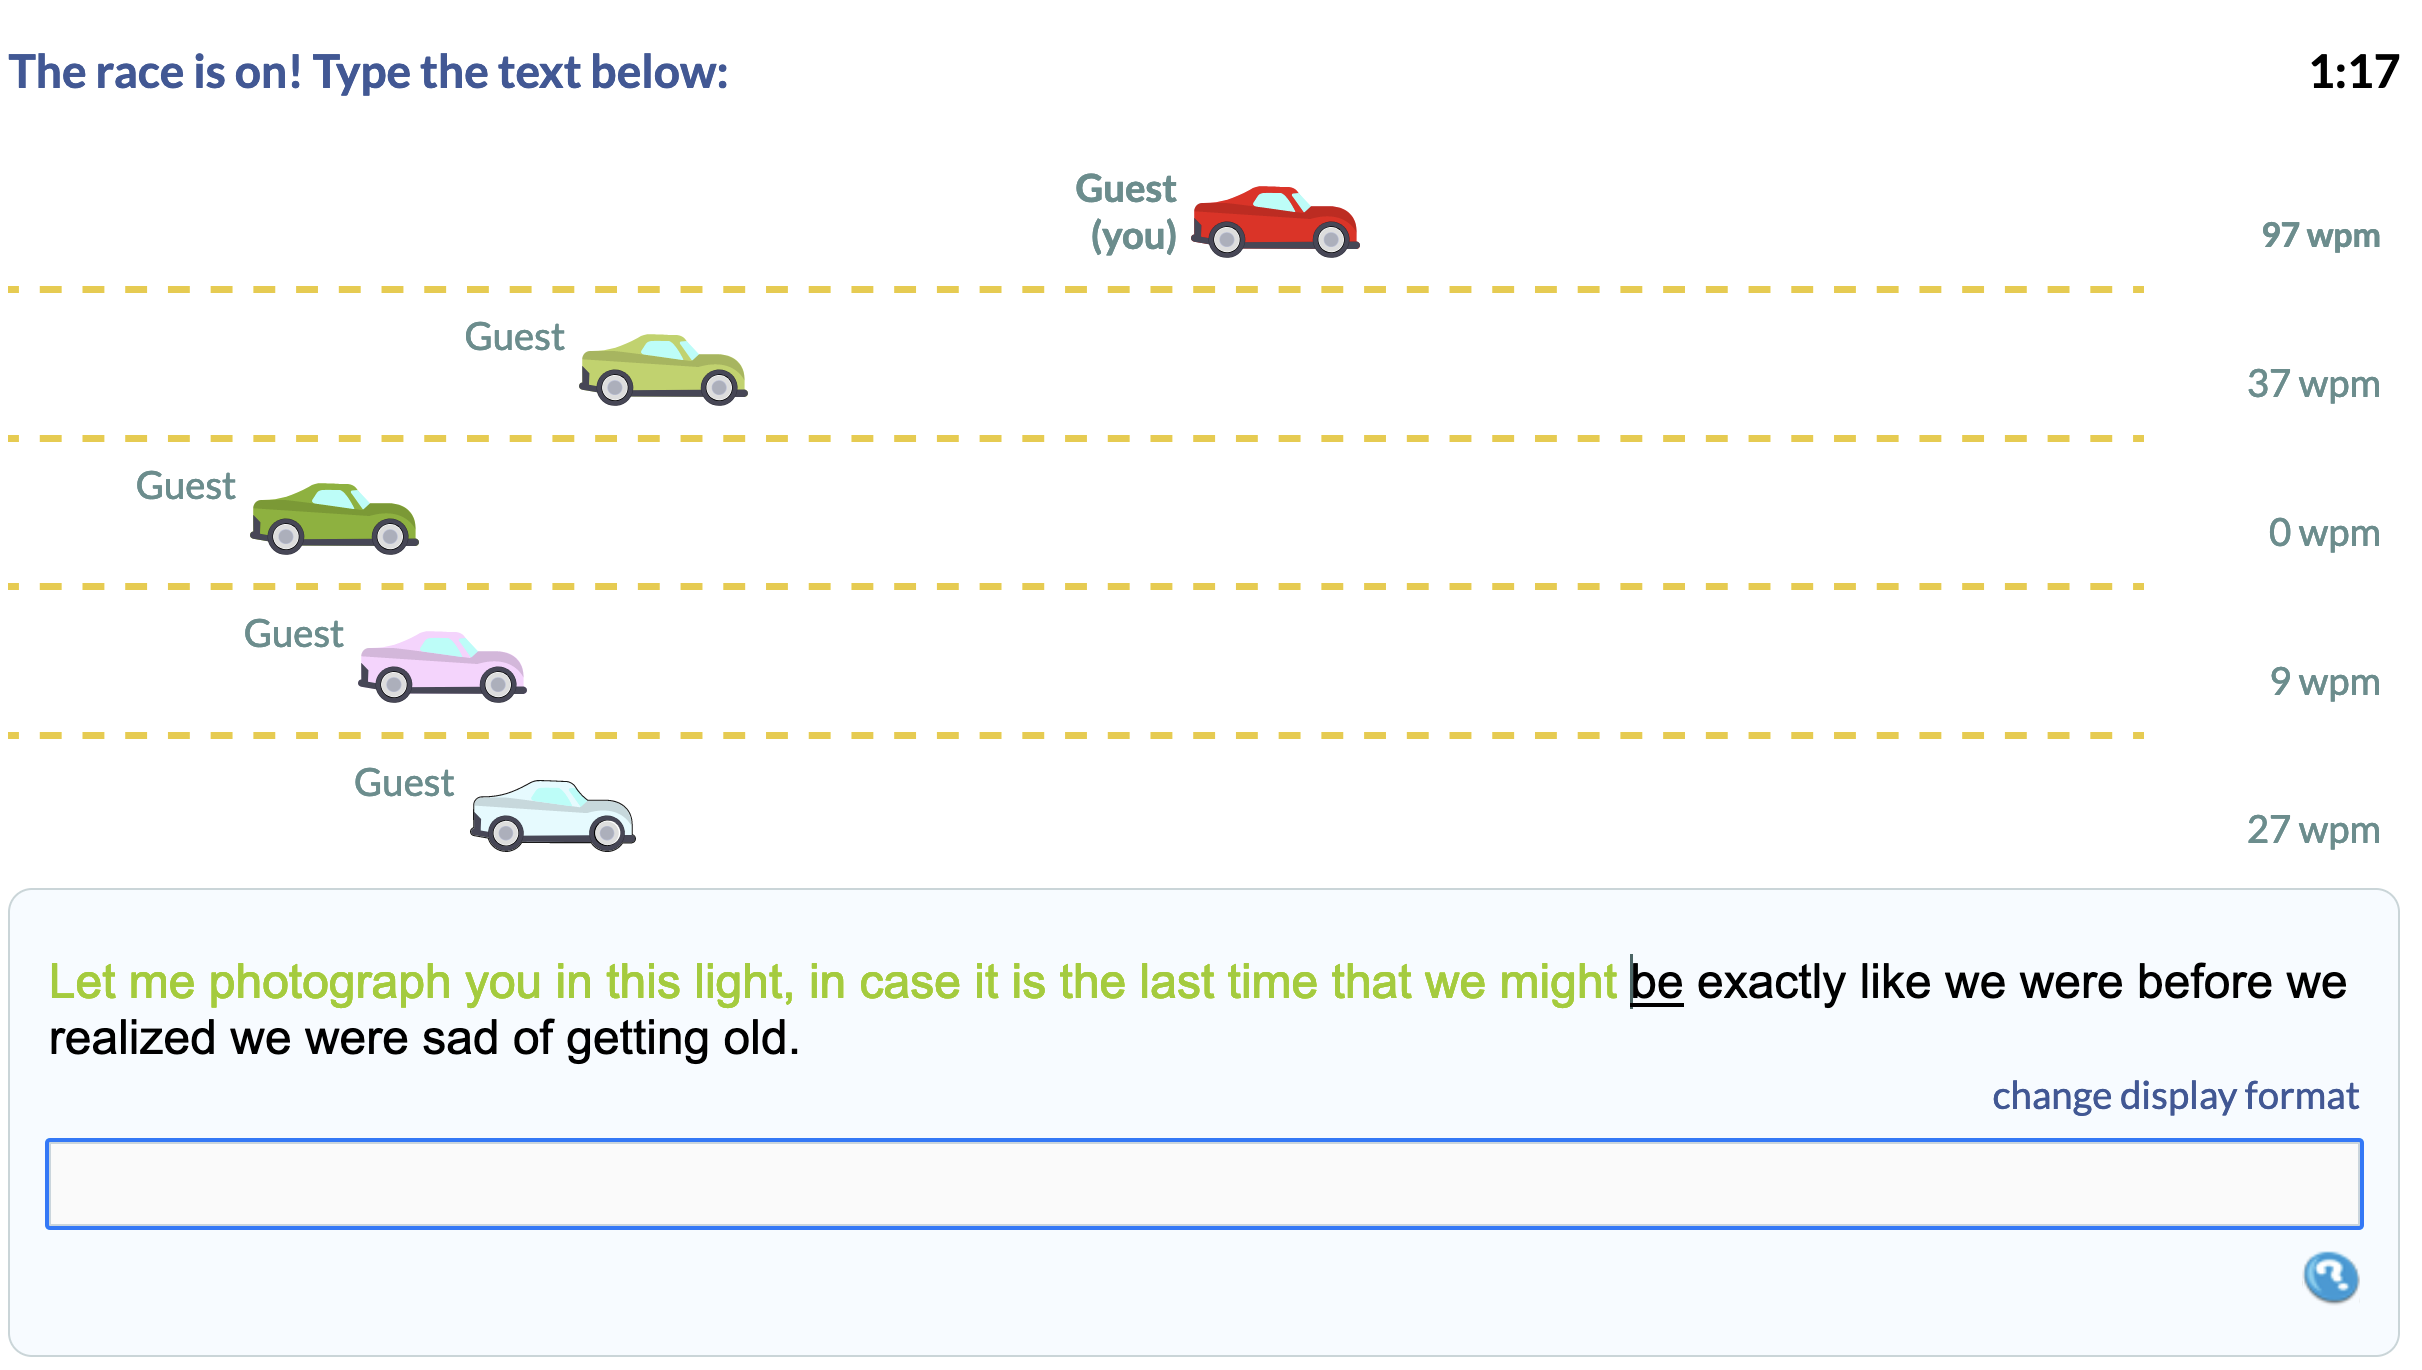
\includegraphics[width=\textwidth]{typeracer.png}
\end{figure}

Your score is a measurement of your average typing speed at the end of the race. Typing speed is measured in the units "words per minute" ("wpm" for short), and each word is defined as five characters.

In TypeRacer, your typing speed determines the types of texts you'll be presented with: a lower typing speed gives you easier texts, while a higher typing speed gives you more difficult texts:

\begin{figure}[hbt!]
	\caption{Two different possible texts in TypeRacer. On the left, an easy text, and on the right, a more difficult text.}
	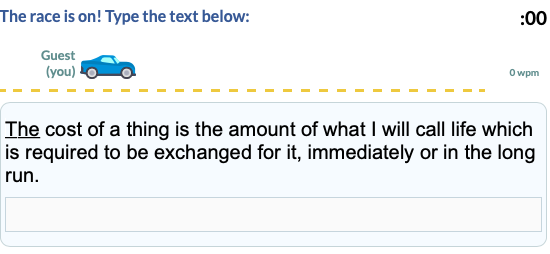
\includegraphics[width=0.5\textwidth]{easy-text.png}
	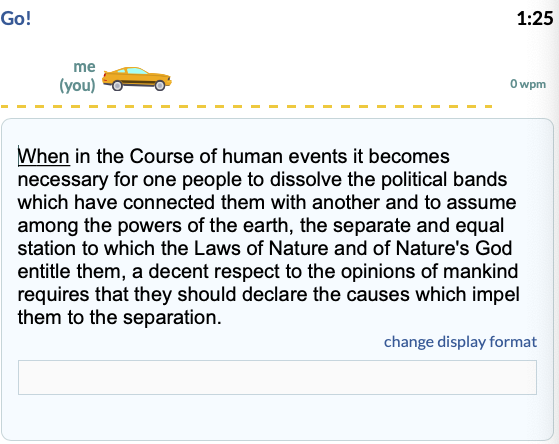
\includegraphics[width=0.5\textwidth]{hard-text.png}
\end{figure}


However, not all texts are created equal. Some texts are harder to type than others, whether it's from having longer, more complex words, frequent capital letters, numbers, etc.

Predicting the difficulty of a text is useful. For example, the typing site that I practice on, TypeRacer, will display different sets of texts depending . For example, these are two quotes that can appear in a TypeRacer race:


Even though Quote 1 is shorter than Quote 2, the difficult word at the start of Quote 1 makes it significantly more difficult to type.

Currently, the way TypeRacer classifies the difficulty of a newly added quote is through . Each player has an average typing speed that is calculated based on their best scores for each quote, and if the

At first, I considered using the length of the text might be to use the length of the text in determining its difficulty. While this works for the two texts shown in Figure 1, it's not a flawless approach. For example, the following two texts are possible texts you can encounter in TypeRacer:

\begin{textexamples}
	\textbf{Text 1}: Supercalifragilisticexpialidocious is Vielle's favorite word to type on TypeRacer.
	\textbf{Text 2}: For someone who was never meant for this world, I must confess I'm suddenly having a hard time leaving it.
\end{textexamples}

Even though Text 1 has fewer characters than Text 2, it is still considerably more difficult to type because of the complex first word.

, but there are many more characteristics of words that affect the speed at which they are typed. For example, one of these characteristics is the fingers you use to type the word.

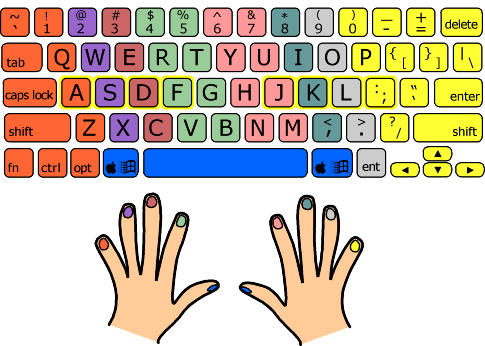
\includegraphics{finger-map.png}

Using this standard finger map, when typing the word \texttt{mummy} on the QWERTY keyboard, you would exclusively use your right index finger to type the entire word, making it significantly slower to type compared to a word like \texttt{there}, which doesn't involve using the same finger to type two consecutive letters.

\begin{textexamples}
\end{textexamples}

The characteristics of how difficult a word is to type extends beyond these two examples, and each characteristic has a different amount of influence on how quickly I type the word. In order to determine the significance of these various characteristics in the difficulty of a word, machine learning can be applied.

\section*{Gathering Data}

In order to create a machine learning algorithm that predicts how fast I can type a certain text based on the text features, we need to collect a large amount of data that includes various texts and the speed at which I type them. Luckily, I've been using TypeRacer for over 5 years now, and over these 5 years I've typed over 8000 texts on my account.

I created a program that automatically scrapes the race data from all my 8000 races and saves them into a file.

\section*{Analyzing Data}


\section*{Predicting Typing Speed}



The purpose of our machine learning algorithm is to find weights for each feature that most accurately predicts the typing data. However, in order to do this, the algorithm needs a way to know how accurate a certain set of weights are.

\subsection*{The Cost Function}

The cost function will inform our machine learning algorithm how accurate its weights are, and more importantly, how to adjust its weights in order to reduce the cost.




\begin{figure}
	\caption{A graph relating the number of capital letters in a word and the speed at which the word is typed.}
	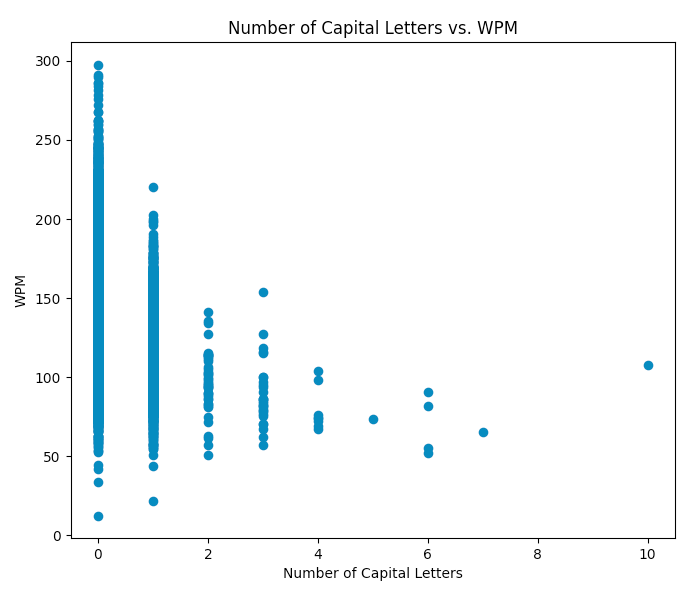
\includegraphics[width=\textwidth]{capital-letters-vs-wpm.png}
\end{figure}

In a word, there are many more features other than the word length and the number of capital letters.

\begin{align*}
	\text{Difficulty} = w_1 * (\text{Feature 1}) + w_2 * (\text{Feature 2}) + ... + \text{Bias}
\end{align*}

For example, if there are two features that influence the difficulty of a word which are the length of the word and the number of capital letters in the word, then the equation would become:

\begin{align*}
	\text{Difficulty} = w_{\text{word length}} * (\text{word length}) + w_{\text{capital letters}} * (\text{\# of capital letters}) + \text{Bias}
\end{align*}

\begin{itemize}
	\item Whether the word is common (1 if the word is included within the top 1000 most common English words, and 0 otherwise).
	\item The number of capital letters in the word.
	\item The number of characters in the word.
	\item The number of sets of "double letters" in the word. For example, the word "sheep" has 1 set of double letters, and the word "bittersweet" has two sets of double letters.
	\item The number of letters in the home row of the keyboard (the row with the letters "asdf" on the QWERTY layout).
	\item The number of letters that require pressing the "Shift" key to type.
	\item The amount of times the same finger is used to type consecutive letters in the word. For example, the word "mummy" requires using the right index finger five times in a row on a QWERTY layout.
	\item The number of letters typed with the left hand.
	\item The number of letters typed with the right hand.
\end{itemize}

\textbf{Note:} The data in the following tables might not match with the data you'd expect on a QWERTY layout, and that's because when analyzing my typing data, I based it off the keyboard layout that I use—the Programmer Dvorak layout—which looks like this:

% \begin{noindent}
\begin{pycode}
word1 = {"word":"profession ","medianWpm":154.134295227525,"isWordCommon":0,"numCapitalLetters":0,"numConsecutiveFingers":1,"numDoubleLetters":1,"numHomeRowLetters":7,"numLeftHandLetters":5,"numNumbers":0,"numRightHandLetters":5,"numShiftedLetters":0,"wordLength":11}

word2 = {"word":"Table, ","medianWpm":136.84411614875188,"isWordCommon":1,"numCapitalLetters":1,"numConsecutiveFingers":0,"numDoubleLetters":0,"numHomeRowLetters":2,"numLeftHandLetters":3,"numNumbers":0,"numRightHandLetters":3,"numShiftedLetters":1,"wordLength":7}

word3 = {"word":"1950s, ","medianWpm":81.3953488372093,"isWordCommon":0,"numCapitalLetters":0,"numConsecutiveFingers":0,"numDoubleLetters":0,"numHomeRowLetters":1,"numLeftHandLetters":4,"numNumbers":4,"numRightHandLetters":2,"numShiftedLetters":4,"wordLength":7}

def get_table_1_row(w):
	return f"""
		\\\\\\hline
		"{w['word']}" &
		{w['wordLength']} &
		{w['numCapitalLetters']} &
		{w['numConsecutiveFingers']} &
		{w['numDoubleLetters']} &
		{w['numHomeRowLetters']}
	"""

def get_table_2_row(w):
	return f"""
		\\\\\\hline
		"{w['word']}" &
		{w['numLeftHandLetters']} &
		{w['numRightHandLetters']} &
		{w['numNumbers']} &
		{w['numShiftedLetters']} &
		{w['isWordCommon']} &
		{"%.2f" % w['medianWpm']}
	"""
\end{pycode}
% \end{noindent}

\begin{table}[hbt!]
	\caption{Three examples of features in words}
	\begin{tabularx}{\linewidth}{|
			p{70pt}|
			>{\RaggedRight}X|
			>{\RaggedRight}X|
			>{\RaggedRight}X|
			>{\RaggedRight}X|
			>{\RaggedRight}X|
			>{\RaggedRight}X|
		}
		\hline

		Word                               &
		\# of Characters                   &
		\# of Capitals                     &
		\# of Same-Finger Consecutive Keys &
		\# of Double Letters               &
		\# of Home Row Letters

		\py{get_table_1_row(word1)}
		\py{get_table_1_row(word2)}
		\py{get_table_1_row(word3)}
		\\\hline
	\end{tabularx}

	\begin{tabularx}{\linewidth}{|
			p{70pt}|
			>{\RaggedRight}X|
			>{\RaggedRight}X|
			>{\RaggedRight}X|
			>{\RaggedRight}X|
			>{\RaggedRight}X|
			>{\RaggedRight}X|
			>{\RaggedRight}X|
		}
		\hline

		Word                          &
		\# of Left Hand Letters       &
		\# of Right Hand Letters      &
		\# of Numbers                 &
		\# of Letters Requiring Shift &
		Is word common?               &
		Median WPM

		\py{get_table_2_row(word1)}
		\py{get_table_2_row(word2)}
		\py{get_table_2_row(word3)}
		\\\hline
	\end{tabularx}
\end{table}


\begin{figure}[hbt!]
	\caption{The Programmer Dvorak Keyboard Layout}
	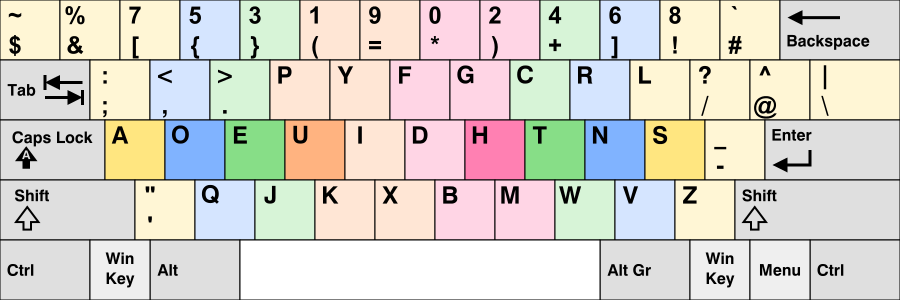
\includegraphics[width=\textwidth]{programmer-dvorak.png}
\end{figure}

\end{document}